\documentclass[11pt,a4paper]{article}

\usepackage[margin=22mm,headheight=14pt]{geometry}

\usepackage{longtable,booktabs,array,hyperref,xcolor,tikz,fancyhdr}

\usepackage{fontspec,xeCJK}

\setmainfont[Ligatures=TeXOff]{Times New Roman}

\setsansfont[Ligatures=TeXOff]{Times New Roman}

\setmonofont[Ligatures=TeXOff,WordSpace={1,1,1}]{Times New Roman}

\setCJKmainfont{Noto Serif CJK SC}

\setCJKsansfont{Noto Serif CJK SC}

\setCJKmonofont{Noto Serif CJK SC}

\XeTeXgenerateactualtext=1

\definecolor{vulcan}{HTML}{BB3E23}

\pgfdeclarelayer{connections}\pgfdeclarelayer{edge labels}\pgfsetlayers{connections,main,edge labels}

\hypersetup{hidelinks}

\newcolumntype{L}[1]{>{\raggedright\arraybackslash}p{#1}}

\setlength{\emergencystretch}{5em}\tolerance=2000\hbadness=10000

\setlength{\parindent}{0pt}\setlength{\parskip}{5pt}

\pagestyle{fancy}\fancyhf{}\fancyhead[L]{\small\sffamily VULCAN}

\fancyhead[R]{\small Product design and verification}\fancyfoot[C]{\thepage}

\begin{document}

{\sffamily\huge\raggedright\textbf{SABLE: Segmented Acknowledged Buffered Link Engine}\par}

{\large Technical Design and Verification Report}\par

\textbf{Developer:} Sufeng Guo\par

15 October 2026 (\allowbreak{}UTC+\allowbreak{}8)\allowbreak{}\par\textcolor{vulcan}{\rule{\textwidth}{0.5pt}}

\begin{abstract}

SABLE is a synthesizable,\allowbreak{} single-clock reliable message transport for four independent streams. Its 64-bit ready/\allowbreak{}valid interfaces carry 1–4096-byte messages,\allowbreak{} fragmented into payloads of at most 256 bytes. Eight-packet selective-repeat windows,\allowbreak{} CRC-32C-protected DATA and acknowledgments,\allowbreak{} bounded out-of-order storage,\allowbreak{} and complete-message reassembly implement reliability entirely in RTL.


The accepted implementation passed 36 required behavioral ledger rows,\allowbreak{} including nine seeded TX,\allowbreak{} RX and bidirectional endpoint experiments. Checker-sensitivity tests detected both injected output defects. Full-capacity generic synthesis retained substantive TX/\allowbreak{}RX hierarchy and storage,\allowbreak{} and source-only clean-directory reproduction passed its independent endpoint smoke and synthesis checks. These results establish software-simulated behavior and generic synthesizability,\allowbreak{} not physical implementation signoff.


\end{abstract}

\section{Architecture and design rationale}

The endpoint explicitly instantiates sable\_\allowbreak{}tx u\_\allowbreak{}tx and sable\_\allowbreak{}rx u\_\allowbreak{}rx. Whole-message TX retention eliminates application replay dependencies; fixed per-stream storage avoids dynamic allocation and cross-stream ownership contention. RX validates a staged frame before assigning persistent storage,\allowbreak{} then copies accepted fragments into reassembly memory in identity order. Independent ACK buffering and whole-frame DATA/\allowbreak{}ACK arbitration break the dependency between a full transmit window and acknowledgment progress. The tradeoff is store-and-forward latency and substantial bounded storage rather than cut-through delivery. TX message storage is 16 KiB; RX uses 8 KiB of packet slots,\allowbreak{} 16 KiB of reassembly storage and 256 bytes of staging,\allowbreak{} totaling 40.25 KiB of payload storage before metadata.

\begin{center}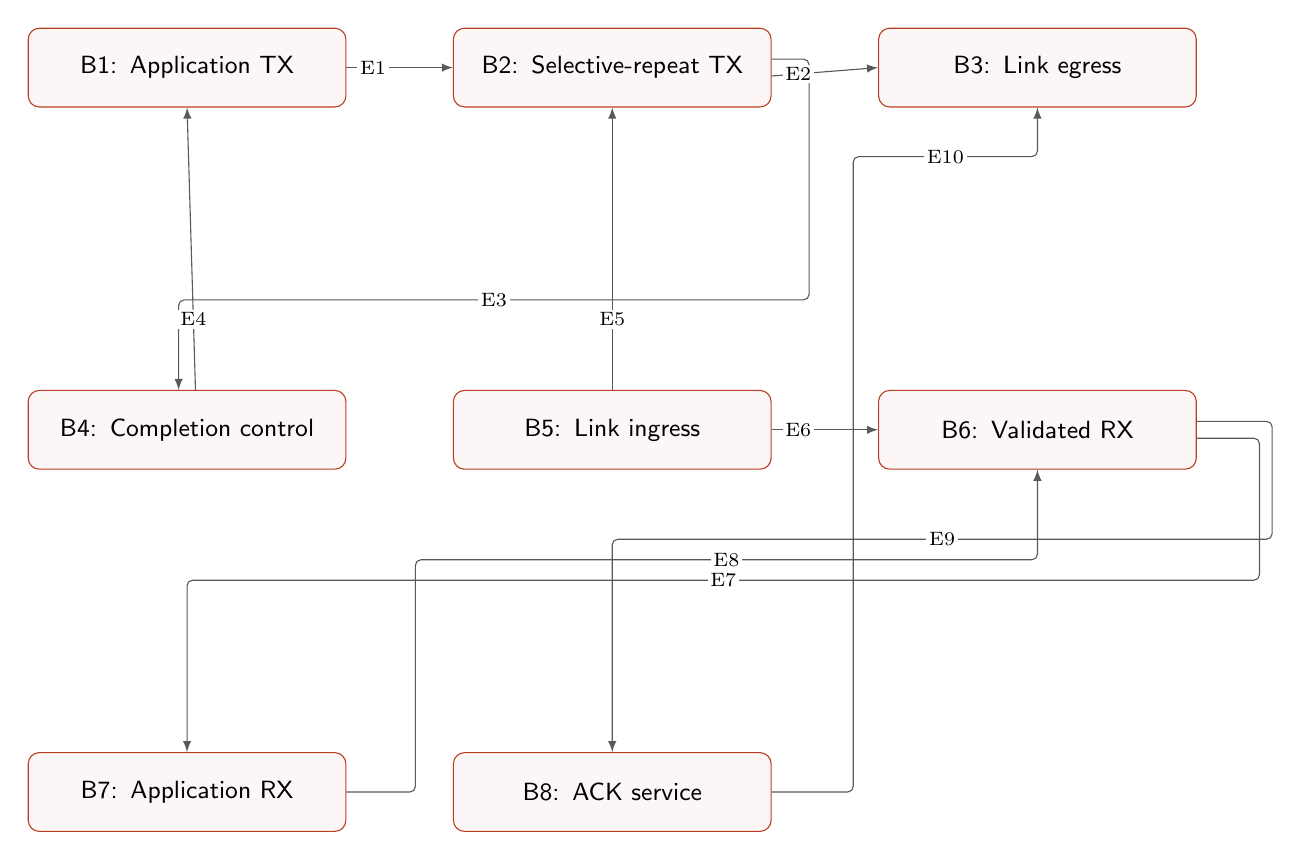
\begin{tikzpicture}[every node/.style={font=\small\sffamily},>=latex]

\node[draw=vulcan,rounded corners,fill=vulcan!4,text width=3.8cm,minimum height=1cm,align=center] (b0) at (0.0,0.0) {B1: Application TX};

\node[draw=vulcan,rounded corners,fill=vulcan!4,text width=3.8cm,minimum height=1cm,align=center] (b1) at (5.4,0.0) {B2: Selective-repeat TX};

\node[draw=vulcan,rounded corners,fill=vulcan!4,text width=3.8cm,minimum height=1cm,align=center] (b2) at (10.8,0.0) {B3: Link egress};

\node[draw=vulcan,rounded corners,fill=vulcan!4,text width=3.8cm,minimum height=1cm,align=center] (b3) at (0.0,-4.6) {B4: Completion control};

\node[draw=vulcan,rounded corners,fill=vulcan!4,text width=3.8cm,minimum height=1cm,align=center] (b4) at (5.4,-4.6) {B5: Link ingress};

\node[draw=vulcan,rounded corners,fill=vulcan!4,text width=3.8cm,minimum height=1cm,align=center] (b5) at (10.8,-4.6) {B6: Validated RX};

\node[draw=vulcan,rounded corners,fill=vulcan!4,text width=3.8cm,minimum height=1cm,align=center] (b6) at (0.0,-9.2) {B7: Application RX};

\node[draw=vulcan,rounded corners,fill=vulcan!4,text width=3.8cm,minimum height=1cm,align=center] (b7) at (5.4,-9.2) {B8: ACK service};

\begin{pgfonlayer}{connections}

\draw[->,black!65] ([yshift=0.000cm]b0.east) -- coordinate[pos=0.25] (e0) ([yshift=0.000cm]b1.west);

\draw[->,black!65] ([yshift=-0.107cm]b1.east) -- coordinate[pos=0.25] (e1) ([yshift=0.000cm]b2.west);

\draw[->,black!65,rounded corners=2pt] ([yshift=0.107cm]b1.east) -- (7.900,0.107) -- (7.900,-2.950) -- coordinate[midway] (e2) (-0.107,-2.950) -- ([xshift=-0.107cm]b3.north);

\draw[->,black!65] ([xshift=0.107cm]b3.north) -- coordinate[pos=0.25] (e3) ([xshift=0.000cm]b0.south);

\draw[->,black!65] ([xshift=0.000cm]b4.north) -- coordinate[pos=0.25] (e4) ([xshift=0.000cm]b1.south);

\draw[->,black!65] ([yshift=0.000cm]b4.east) -- coordinate[pos=0.25] (e5) ([yshift=0.000cm]b5.west);

\draw[->,black!65,rounded corners=2pt] ([yshift=-0.107cm]b5.east) -- (13.620,-4.707) -- (13.620,-6.510) -- coordinate[midway] (e6) (0.000,-6.510) -- ([xshift=0.000cm]b6.north);

\draw[->,black!65,rounded corners=2pt] ([yshift=0.000cm]b6.east) -- (2.900,-9.200) -- (2.900,-6.250) -- coordinate[midway] (e7) (10.800,-6.250) -- ([xshift=0.000cm]b5.south);

\draw[->,black!65,rounded corners=2pt] ([yshift=0.107cm]b5.east) -- (13.780,-4.493) -- (13.780,-5.990) -- coordinate[midway] (e8) (5.400,-5.990) -- ([xshift=0.000cm]b7.north);

\draw[->,black!65,rounded corners=2pt] ([yshift=0.000cm]b7.east) -- (8.460,-9.200) -- (8.460,-1.130) -- coordinate[midway] (e9) (10.800,-1.130) -- ([xshift=0.000cm]b2.south);

\end{pgfonlayer}

\begin{pgfonlayer}{edge labels}

\node[fill=white,inner sep=1pt,font=\scriptsize] at (e0) {E1};

\node[fill=white,inner sep=1pt,font=\scriptsize] at (e1) {E2};

\node[fill=white,inner sep=1pt,font=\scriptsize] at (e2) {E3};

\node[fill=white,inner sep=1pt,font=\scriptsize] at (e3) {E4};

\node[fill=white,inner sep=1pt,font=\scriptsize] at (e4) {E5};

\node[fill=white,inner sep=1pt,font=\scriptsize] at (e5) {E6};

\node[fill=white,inner sep=1pt,font=\scriptsize] at (e6) {E7};

\node[fill=white,inner sep=1pt,font=\scriptsize] at (e7) {E8};

\node[fill=white,inner sep=1pt,font=\scriptsize] at (e8) {E9};

\node[fill=white,inner sep=1pt,font=\scriptsize] at (e9) {E10};

\end{pgfonlayer}

\end{tikzpicture}\end{center}

{\small Functional block map, not a gate-level netlist. Edge identifiers match the directed relationships below. Crossings do not denote junctions; separate attachment points preserve arrow directions.}

{\small\begin{longtable}{@{}L{0.24\textwidth}L{0.7\textwidth}@{}}\toprule

\textbf{Block} & \textbf{Responsibility}\\\midrule\endhead

B1: Application TX & Collects independently interleaved application streams into four 4096-byte message banks and reserves each message's complete identity range.\\[3pt]

B2: Selective-repeat TX & Within u\_\allowbreak{}tx,\allowbreak{} performs fragmentation,\allowbreak{} eight-position window scheduling,\allowbreak{} DATA serialization,\allowbreak{} CRC generation,\allowbreak{} ACK validation,\allowbreak{} timers and retry accounting.\\[3pt]

B3: Link egress & Alternates eligible DATA and ACK frames,\allowbreak{} holds ownership through the tail,\allowbreak{} and uses a registered shadow beat retired only by the public link handshake.\\[3pt]

B4: Completion control & Maintains four completion mailboxes,\allowbreak{} fair status arbitration and sticky per-stream failure or identity-exhaustion indications.\\[3pt]

B5: Link ingress & Registers received beats and locks routing to DATA or ACK processing for the entire frame. Unframed residual beats are discarded.\\[3pt]

B6: Validated RX & Within u\_\allowbreak{}rx,\allowbreak{} checks structure,\allowbreak{} session and CRC in 256-byte staging,\allowbreak{} commits eight packet slots per stream,\allowbreak{} and performs ordered reassembly into four 4096-byte banks.\\[3pt]

B7: Application RX & Publishes complete messages through registered,\allowbreak{} beat-level round-robin arbitration; each bank remains owned until its application tail handshake.\\[3pt]

B8: ACK service & Queues 32 stream/\allowbreak{}identity entries independently of DATA windows and serializes protected four-beat ACK frames. An active ACK context is separate from FIFO storage.\\[3pt]

\bottomrule\end{longtable}}

{\small\begin{longtable}{@{}L{0.24\textwidth}L{0.7\textwidth}@{}}\toprule

\textbf{Directed relationship} & \textbf{Meaning}\\\midrule\endhead

E1: B1 to B2 & Complete retained messages\\[3pt]

E2: B2 to B3 & DATA frames\\[3pt]

E3: B2 to B4 & Terminal results and faults\\[3pt]

E4: B4 to B1 & Release after status and frame drain\\[3pt]

E5: B5 to B2 & Received ACK frames\\[3pt]

E6: B5 to B6 & Received DATA frames\\[3pt]

E7: B6 to B7 & Complete retained messages\\[3pt]

E8: B7 to B6 & Tail handshake releases bank\\[3pt]

E9: B6 to B8 & Accepted or duplicate identities\\[3pt]

E10: B8 to B3 & Protected ACK frames\\[3pt]

\bottomrule\end{longtable}}

\section{Interfaces and configuration}

{\small\begin{longtable}{@{}L{0.2\textwidth}L{0.12\textwidth}L{0.1\textwidth}L{0.48\textwidth}@{}}\toprule

\textbf{Signal /\allowbreak{} group} & \textbf{Direction} & \textbf{Width} & \textbf{Contract}\\\midrule\endhead

clk,\allowbreak{} rst,\allowbreak{} session\_\allowbreak{}id & Input & 1,\allowbreak{} 1,\allowbreak{} 32 bits & One rising-edge clock and active-high synchronous state reset. Session is sampled on reset and remains stable during operation. Public outputs,\allowbreak{} including ready,\allowbreak{} are masked to zero while rst is asserted.\\[3pt]

s\_\allowbreak{}msg\_\allowbreak{}*\allowbreak{} & Input; ready output & data 64; keep 8; stream 2; len 13; valid/\allowbreak{}ready/\allowbreak{}first/\allowbreak{}last 1 bit each & Application transmit channel. Streams may interleave by beat,\allowbreak{} but each stream owns at most one unfinished message. Length is constant per message; keep is low-contiguous and equals ff on non-tail beats.\\[3pt]

m\_\allowbreak{}msg\_\allowbreak{}*\allowbreak{} & Output; ready input & data 64; keep 8; stream 2; len 13; valid/\allowbreak{}ready/\allowbreak{}first/\allowbreak{}last 1 bit each & Complete-message receive channel. Output beats may interleave streams; consumers reconstruct each stream separately. A 1–8-byte message has first and last asserted together.\\[3pt]

m\_\allowbreak{}status\_\allowbreak{}*\allowbreak{},\allowbreak{} tx\_\allowbreak{}failed,\allowbreak{} session\_\allowbreak{}exhausted & Output; m\_\allowbreak{}status\_\allowbreak{}ready input & stream/\allowbreak{}code 2 bits each; valid/\allowbreak{}ready 1 bit each; fault vectors 4 bits each & One terminal status per accepted message unless reset cancels it: code 0 is ACKED,\allowbreak{} code 1 UNACKNOWLEDGED. Sticky vector bits identify streams closed by retry failure or insufficient remaining identities.\\[3pt]

link\_\allowbreak{}tx\_\allowbreak{}*\allowbreak{},\allowbreak{} link\_\allowbreak{}rx\_\allowbreak{}*\allowbreak{} & Transmit output and receive input; ready reverses direction & data 64; keep 8; valid/\allowbreak{}ready/\allowbreak{}first/\allowbreak{}last 1 bit each & Framed wire channels with no external stream sideband. Stream,\allowbreak{} session and identity are protected header fields. Transfers occur only on pre-edge valid \&\& ready outside reset.\\[3pt]

Standalone protocol channels & TX: m\_\allowbreak{}data output,\allowbreak{} s\_\allowbreak{}ack input; RX: s\_\allowbreak{}data input,\allowbreak{} m\_\allowbreak{}ack output & 64-bit data,\allowbreak{} 8-bit keep,\allowbreak{} 1-bit handshake/\allowbreak{}framing signals & sable\_\allowbreak{}tx and sable\_\allowbreak{}rx expose the same DATA/\allowbreak{}ACK format independently for integration and model-based testing. All public ports are unsigned.\\[3pt]

\bottomrule\end{longtable}}

{\small\begin{longtable}{@{}L{0.23\textwidth}L{0.12\textwidth}L{0.57\textwidth}@{}}\toprule

\textbf{Parameter} & \textbf{Default} & \textbf{Meaning /\allowbreak{} supported values}\\\midrule\endhead

TIMEOUT\_\allowbreak{}CYCLES & 4096 & Integer 1–65535 on TX and endpoint. Counts after actual DATA tail transfer,\allowbreak{} excluding active serialization; expiry creates a scheduling candidate.\\[3pt]

MAX\_\allowbreak{}RETRIES & 4 & Integer 0–15 on TX and endpoint. Counts retransmissions beyond the initial send; default permits five total transmissions.\\[3pt]

GENERATION\_\allowbreak{}BITS & 24 & Integer 1–24 on all modules. Identity capacity is 2\textasciicircum{}(\allowbreak{}8+\allowbreak{}GENERATION\_\allowbreak{}BITS)\allowbreak{} packets per stream per session; unused wire generation bits must be zero.\\[3pt]

Fixed product capacities & 4 streams; 8 window/\allowbreak{}receive slots per stream; 4096-byte messages; 32 ACK FIFO entries & Not capacity-reduction parameters. Illegal configurable values are explicitly rejected rather than clamped.\\[3pt]

\bottomrule\end{longtable}}

\section{Behavior and corner cases}

\subsection{Wire representation and integrity}

Frames contain three full 64-bit header beats,\allowbreak{} DATA payload beats,\allowbreak{} and a separate CRC tail. Header byte offsets are: 0–2 constants 53/\allowbreak{}42/\allowbreak{}01 hexadecimal; 3 type (\allowbreak{}DATA=\allowbreak{}0,\allowbreak{} ACK=\allowbreak{}1)\allowbreak{}; 4 stream; 5 SOM/\allowbreak{}EOM bits; 6–7 payload length; 8–11 session; 12 sequence; 13–15 generation; 16–17 message length; 18–19 byte offset; 20–23 zero. Integers are little-endian,\allowbreak{} low byte lane first. ACK retains only stream,\allowbreak{} session and identity,\allowbreak{} with other variable fields zero. Headers use keep=\allowbreak{}ff; CRC uses keep=\allowbreak{}0f,\allowbreak{} zero upper 32 bits and exclusive last. DATA requires 5–36 beats; ACK always requires four.

\subsection{CRC-32C}

Castagnoli parameters are polynomial 1edc6f41,\allowbreak{} reflected polynomial 82f63b78,\allowbreak{} init/\allowbreak{}xorout ffffffff,\allowbreak{} refin/\allowbreak{}refout true. Bytes follow wire order and enter least-significant bit first. Coverage includes all 24 header bytes and valid payload bytes,\allowbreak{} excluding CRC and padding. The CRC is transmitted little-endian. The standard ASCII 123456789 result is e3069283. Structural validation remains necessary even when CRC is valid.

\subsection{Fragmentation and selective repeat}

A message requires ceil(\allowbreak{}length/\allowbreak{}256)\allowbreak{} fragments,\allowbreak{} at most 16. Offset is a multiple of 256 and payload length is min(\allowbreak{}256,\allowbreak{}length−offset)\allowbreak{}. New identities cannot advance more than seven positions beyond the oldest unacknowledged identity; intermediate ACKs do not open a ninth position. CRC-valid ACKs must match a transmitted active identity. Matching ACK wins over simultaneous timeout. An ACK during retransmission retires the identity while the already-started frame drains without releasing its payload prematurely.

\subsection{Receive ownership and resource pressure}

Any valid in-window fragment can establish a message using identity minus fragment index. Eight slots retain arbitrary arrival order relative to next-to-copy; ordered copying produces one complete message without duplicate delivery. Retained,\allowbreak{} copied and committed older identities can regenerate ACKs. Invalid,\allowbreak{} too-far-future or resource-rejected frames drain without positive acknowledgment. Full ACK storage drops only new ACK requests,\allowbreak{} not accepted DATA; duplicates regenerate lost ACKs. Simultaneous FIFO enqueue/\allowbreak{}dequeue preserves occupancy and can use the released entry.

\subsection{Timing and fairness}

Every producer has a final holding register; stalled valid data and metadata remain unchanged. A state commit at edge k can first load a dependent final output at k+\allowbreak{}1 and transfer it at k+\allowbreak{}2,\allowbreak{} with additional processing latency permitted. TX rotates whole DATA frames across four eligible streams; endpoint arbitration alternates DATA and ACK frames; RX copy,\allowbreak{} application output and status arbitration are fair at their respective operation boundaries. These bounds assume downstream service. One shared ready can stall the selected application beat,\allowbreak{} and an input source holding an unavailable stream can block its own multiplexed input.

\subsection{Completion and failure}

ACKED means every fragment was accepted and retained by the peer in the current session,\allowbreak{} not necessarily consumed by its application or persisted across reset. Retry exhaustion reports UNACKNOWLEDGED and closes only that TX stream until reset. It does not imply non-delivery. Message storage is reusable only after completion handshake and any active redundant transmission drains.

\subsection{Reset and identity lifetime}

Paired reset cancels partial messages,\allowbreak{} windows,\allowbreak{} queues,\allowbreak{} statuses and partial outputs. Both endpoints require the same fresh session; interrupted receive messages must be discarded by the application. Sequence 255 advances to zero with generation increment. Full identities never wrap: TX atomically checks the entire new message allocation and refuses insufficient space. Default lifetime is 2\textasciicircum{}32 packets per stream; GENERATION\_\allowbreak{}BITS=\allowbreak{}1 allows 512. Old-session frames cannot complete new transactions.

\section{Verification methods and measured results}

\subsection{Independent behavioral correctness and bounded progress}

\textbf{Method.} Public-pin Python wire/\allowbreak{}byte oracles separately checked RTL TX,\allowbreak{} RTL RX and paired endpoints for seeds 17,\allowbreak{} 89 and 203,\allowbreak{} with stalls,\allowbreak{} fault decisions and a 200000-cycle cap. Lengths were 1,\allowbreak{} 2,\allowbreak{} 7,\allowbreak{} 8,\allowbreak{} 9,\allowbreak{} 255,\allowbreak{} 256,\allowbreak{} 257,\allowbreak{} 511,\allowbreak{} 512,\allowbreak{} 513,\allowbreak{} 2047,\allowbreak{} 2048,\allowbreak{} 2049,\allowbreak{} 4095 and 4096 bytes.

\textbf{Result.} 36/\allowbreak{}36 ledger rows passed: nine seeded experiments and 27 directed/\allowbreak{}parameter rows. TX/\allowbreak{}RX/\allowbreak{}endpoint cycles were respectively 19172/\allowbreak{}17389/\allowbreak{}41127 for seed 17,\allowbreak{} 19177/\allowbreak{}17347/\allowbreak{}42989 for 89,\allowbreak{} and 19204/\allowbreak{}17783/\allowbreak{}40779 for 203. Each endpoint seed compared 44 delivered messages,\allowbreak{} 44 statuses and 57914 receive bytes. The complete ledger and fault records are retained under evidence/\allowbreak{}behavior/\allowbreak{}behavior-20261015T105439Z-f3730c4f/\allowbreak{}.

{\small Evidence: E029,\allowbreak{} E008,\allowbreak{} E012,\allowbreak{} E014}

\subsection{Effective windows,\allowbreak{} corruption rejection and finite-resource recovery}

\textbf{Method.} Frozen ACKs measured actual outstanding packets; independent decoding checked CRC and malformed frames. Directed scenarios exercised reverse-order slots,\allowbreak{} FIFO/\allowbreak{}mailbox pressure,\allowbreak{} arbitration,\allowbreak{} timers and failure ambiguity.

\textbf{Result.} Eight unacknowledged packets per stream and 32 aggregate were observed; the oldest hole blocked the ninth. All three endpoint seeds observed DATA and ACK reordering and each received 96 detected-invalid frames. ACK saturation retained 33 acknowledgments across FIFO plus active context and regenerated a dropped request. Retry exhaustion produced exactly five sends with four retries while another stream completed.

{\small Evidence: E029,\allowbreak{} E008,\allowbreak{} E011,\allowbreak{} E012}

\subsection{Reset phase coverage,\allowbreak{} wrap and parameter boundaries}

\textbf{Method.} Handshake-witnessed interruption tested TX/\allowbreak{}RX payload,\allowbreak{} stalled TX CRC,\allowbreak{} partial ACK and endpoint ingress/\allowbreak{}egress locks,\allowbreak{} followed by residual and old-session replay. Separate tests exercised sequence wrap,\allowbreak{} identity exhaustion and parameter boundaries.

\textbf{Result.} All six phase-witness cases passed,\allowbreak{} supplementing three cancellation cases. Default sequence wrap rejected late old DATA/\allowbreak{}ACK effects; shortened identity tests covered 512-packet exhaustion and whole-message refusal with only eight identities remaining. Eight legal parameter tuples elaborated and reset; six out-of-range values were explicitly rejected. Observable phase witnesses close the coverage gap that elapsed wait offsets alone could not establish.

{\small Evidence: E029,\allowbreak{} E008,\allowbreak{} E011}

\subsection{Comparator sensitivity to real incorrect outputs}

\textbf{Method.} Unchanged RTL ran through the normal simulator/\allowbreak{}comparison entry,\allowbreak{} with one accepted application byte and one actual completion handshake independently corrupted.

\textbf{Result.} Both children exited 1 for the intended semantic mismatch: byte 213 versus 212 and completion 1 versus 0. The parent passed after recognizing both failures and retained injection evidence; compilation failures were not substituted.

{\small Evidence: E030,\allowbreak{} E017,\allowbreak{} E014}

\subsection{Full-capacity generic synthesizability}

\textbf{Method.} Yosys 0.33 executed hierarchy checking,\allowbreak{} complete coarse synthesis with memory retention,\allowbreak{} check -assert,\allowbreak{} statistics and JSON export for the default endpoint.

\textbf{Result.} Passed with u\_\allowbreak{}tx/\allowbreak{}u\_\allowbreak{}rx retained,\allowbreak{} no accepted latch or blackbox,\allowbreak{} 24 generic memory cells,\allowbreak{} 132344 TX memory bits and 200420 RX memory bits. Representative generic counts include 5527 mux cells and 357 ALU cells. The script uses exclusive end label begin:fine to include coarse synthesis and disables optional SAT sharing after its retained timeout; neither adjustment reduces resources. Memories were not technology-mapped.

{\small Evidence: E031,\allowbreak{} E016,\allowbreak{} E008}

\subsection{Source-only reproducibility}

\textbf{Method.} Declared sources were hash-checked in a fresh project-local directory; independent endpoint smoke and default-capacity synthesis ran from that directory without copied evidence,\allowbreak{} binaries or private state.

\textbf{Result.} Passed. The 1/\allowbreak{}9/\allowbreak{}257/\allowbreak{}4096-byte four-stream smoke completed in 14797 cycles with 32 messages,\allowbreak{} 32 statuses and 34904 compared receive bytes. This is a scoped clean-reproduction check,\allowbreak{} not a second execution of the complete behavioral matrix. Recorded tools were Python 3.12.3,\allowbreak{} Icarus/\allowbreak{}vvp 12.0 and Yosys 0.33.

{\small Evidence: E032,\allowbreak{} E017,\allowbreak{} E008}

\section{Integration and use}

Compile all rtl/\allowbreak{}*\allowbreak{}.sv with sable\_\allowbreak{}endpoint as top,\allowbreak{} or use standalone sable\_\allowbreak{}tx/\allowbreak{}sable\_\allowbreak{}rx. Exact contracts and storage ownership are in design/\allowbreak{}SPEC.md and design/\allowbreak{}ARCHITECTURE.md. README.md and tests/\allowbreak{}README.md identify MIT-licensed sources,\allowbreak{} generated outputs,\allowbreak{} dependencies and evidence.


Assert rst across at least one rising edge on both endpoints with a fresh common session\_\allowbreak{}id. Keep session stable thereafter. Reconstruct receive messages per stream,\allowbreak{} obey stall stability and contiguous keep,\allowbreak{} consume statuses,\allowbreak{} and initiate paired new-session reset after failure or identity exhaustion.


From the project root,\allowbreak{} run \texttt{python3 tests/\allowbreak{}verify.py behavior --seeds 17 89 203 --max-cycles 200000 --out evidence/\allowbreak{}behavior} and \texttt{python3 tests/\allowbreak{}verify.py negative --out evidence/\allowbreak{}negative}.


Run \texttt{python3 tests/\allowbreak{}verify.py synthesis --out evidence/\allowbreak{}synthesis} and \texttt{python3 tests/\allowbreak{}verify.py reproduce --out evidence/\allowbreak{}reproduce}. Existing Python 3,\allowbreak{} iverilog,\allowbreak{} vvp and Yosys are required; no downloaded packages are needed. Each invocation creates fresh retained evidence with source hashes,\allowbreak{} command receipts,\allowbreak{} raw logs and outcomes.


\section{Limitations and acceptance boundary}

Success requires bounded fairness: service at least every two cycles,\allowbreak{} source beats within four cycles,\allowbreak{} receive blocking at most 512 cycles before regular service,\allowbreak{} extra link delay at most 64 cycles,\allowbreak{} at most two unavailable DATA/\allowbreak{}ACK events per identity and finite duplication/\allowbreak{}reordering. Permanent loss or backpressure is not covered; short timeout configurations need not satisfy the default success envelope.


CRC detects errors but provides neither authentication nor protection against every possible multi-bit corruption. Correct-content guarantees exclude undetected collisions. Ordinary injected faults preserve finite canonical framing; an indefinitely missing last beat is outside recovery guarantees.


Session uniqueness is an integration responsibility. Single-end reset requires paired reset to a new session; no nonvolatile transaction identity or exactly-once persistence across reset is provided.


The evidence is finite simulation and generic synthesis,\allowbreak{} not exhaustive formal proof,\allowbreak{} measured throughput,\allowbreak{} operating-frequency qualification,\allowbreak{} technology area,\allowbreak{} power,\allowbreak{} timing closure,\allowbreak{} board validation or silicon signoff. No TCP,\allowbreak{} RDMA,\allowbreak{} PCIe or physical-network compatibility is implemented.


Preparation failures and repairs remain retained rather than counted as passes. Current results distinguish compilation,\allowbreak{} executed self-checks and independently accepted engineering. Tool/\allowbreak{}call billing cost was unavailable.


\appendix\section{Source inventory}

Production inventory: 3 Verilog/\allowbreak{}SystemVerilog files; 948 nonblank,\allowbreak{} non-comment lines. Source size is not a correctness or quality metric.

{\small\begin{longtable}{@{}L{0.61\textwidth}L{0.15\textwidth}L{0.15\textwidth}@{}}\toprule

\textbf{Production file} & \textbf{Physical lines} & \textbf{Code lines}\\\midrule\endhead

rtl/\allowbreak{}sable\_\allowbreak{}endpoint.sv & 147 & 141\\[3pt]

rtl/\allowbreak{}sable\_\allowbreak{}rx.sv & 405 & 393\\[3pt]

rtl/\allowbreak{}sable\_\allowbreak{}tx.sv & 427 & 414\\[3pt]

\bottomrule\end{longtable}}

\section{Verification record index}

{\small\begin{longtable}{@{}L{0.57\textwidth}L{0.16\textwidth}L{0.17\textwidth}@{}}\toprule

\textbf{Recorded check} & \textbf{Outcome} & \textbf{Execution time (\allowbreak{}s)\allowbreak{}}\\\midrule\endhead

behavior & passed & 58.554\\[3pt]

negative & passed & 1.995\\[3pt]

synthesis & passed & 62.108\\[3pt]

clean-reproduction & passed & 68.156\\[3pt]

\bottomrule\end{longtable}}

Execution times include tool and provider waiting; they are not hardware latency or model utilization.

{\small\begin{longtable}{@{}L{0.12\textwidth}L{0.82\textwidth}@{}}\toprule

\textbf{Reference} & \textbf{Original project-relative record}\\\midrule\endhead

E008 & tests/\allowbreak{}README.md\\[3pt]

E011 & tests/\allowbreak{}directed.py\\[3pt]

E012 & tests/\allowbreak{}model.py\\[3pt]

E014 & tests/\allowbreak{}scenarios.py\\[3pt]

E016 & tests/\allowbreak{}synthesis.py\\[3pt]

E017 & tests/\allowbreak{}verify.py\\[3pt]

E029 & .vulcan/\allowbreak{}engineering/\allowbreak{}run-0001/\allowbreak{}attempt-0009/\allowbreak{}stdout.log\\[3pt]

E030 & .vulcan/\allowbreak{}engineering/\allowbreak{}run-0001/\allowbreak{}attempt-0010/\allowbreak{}stdout.log\\[3pt]

E031 & .vulcan/\allowbreak{}engineering/\allowbreak{}run-0001/\allowbreak{}attempt-0011/\allowbreak{}stdout.log\\[3pt]

E032 & .vulcan/\allowbreak{}engineering/\allowbreak{}run-0001/\allowbreak{}attempt-0012/\allowbreak{}stdout.log\\[3pt]

\bottomrule\end{longtable}}

\section{Document provenance}

Engineering was independently accepted for the recorded source and evidence identity. This is not exhaustive proof, hardware deployment or physical signoff. The companion REPORT.md records the exact report approval and source manifest, and links the English/Chinese journeys containing original failures and interventions. A report number identifies a generation attempt, not a new hardware revision.

Developer attribution is explicitly supplied project metadata, not inferred affiliation or institutional endorsement.

\end{document}
